% Options for packages loaded elsewhere
\PassOptionsToPackage{unicode}{hyperref}
\PassOptionsToPackage{hyphens}{url}
\PassOptionsToPackage{dvipsnames,svgnames,x11names}{xcolor}
%
\documentclass[
  letterpaper,
  DIV=11,
  numbers=noendperiod]{scrartcl}

\usepackage{amsmath,amssymb}
\usepackage{lmodern}
\usepackage{iftex}
\ifPDFTeX
  \usepackage[T1]{fontenc}
  \usepackage[utf8]{inputenc}
  \usepackage{textcomp} % provide euro and other symbols
\else % if luatex or xetex
  \usepackage{unicode-math}
  \defaultfontfeatures{Scale=MatchLowercase}
  \defaultfontfeatures[\rmfamily]{Ligatures=TeX,Scale=1}
\fi
% Use upquote if available, for straight quotes in verbatim environments
\IfFileExists{upquote.sty}{\usepackage{upquote}}{}
\IfFileExists{microtype.sty}{% use microtype if available
  \usepackage[]{microtype}
  \UseMicrotypeSet[protrusion]{basicmath} % disable protrusion for tt fonts
}{}
\makeatletter
\@ifundefined{KOMAClassName}{% if non-KOMA class
  \IfFileExists{parskip.sty}{%
    \usepackage{parskip}
  }{% else
    \setlength{\parindent}{0pt}
    \setlength{\parskip}{6pt plus 2pt minus 1pt}}
}{% if KOMA class
  \KOMAoptions{parskip=half}}
\makeatother
\usepackage{xcolor}
\setlength{\emergencystretch}{3em} % prevent overfull lines
\setcounter{secnumdepth}{5}
% Make \paragraph and \subparagraph free-standing
\ifx\paragraph\undefined\else
  \let\oldparagraph\paragraph
  \renewcommand{\paragraph}[1]{\oldparagraph{#1}\mbox{}}
\fi
\ifx\subparagraph\undefined\else
  \let\oldsubparagraph\subparagraph
  \renewcommand{\subparagraph}[1]{\oldsubparagraph{#1}\mbox{}}
\fi


\providecommand{\tightlist}{%
  \setlength{\itemsep}{0pt}\setlength{\parskip}{0pt}}\usepackage{longtable,booktabs,array}
\usepackage{calc} % for calculating minipage widths
% Correct order of tables after \paragraph or \subparagraph
\usepackage{etoolbox}
\makeatletter
\patchcmd\longtable{\par}{\if@noskipsec\mbox{}\fi\par}{}{}
\makeatother
% Allow footnotes in longtable head/foot
\IfFileExists{footnotehyper.sty}{\usepackage{footnotehyper}}{\usepackage{footnote}}
\makesavenoteenv{longtable}
\usepackage{graphicx}
\makeatletter
\def\maxwidth{\ifdim\Gin@nat@width>\linewidth\linewidth\else\Gin@nat@width\fi}
\def\maxheight{\ifdim\Gin@nat@height>\textheight\textheight\else\Gin@nat@height\fi}
\makeatother
% Scale images if necessary, so that they will not overflow the page
% margins by default, and it is still possible to overwrite the defaults
% using explicit options in \includegraphics[width, height, ...]{}
\setkeys{Gin}{width=\maxwidth,height=\maxheight,keepaspectratio}
% Set default figure placement to htbp
\makeatletter
\def\fps@figure{htbp}
\makeatother

\KOMAoption{captions}{tableheading}
\makeatletter
\makeatother
\makeatletter
\@ifpackageloaded{caption}{}{\usepackage{caption}}
\AtBeginDocument{%
\ifdefined\contentsname
  \renewcommand*\contentsname{Table of contents}
\else
  \newcommand\contentsname{Table of contents}
\fi
\ifdefined\listfigurename
  \renewcommand*\listfigurename{List of Figures}
\else
  \newcommand\listfigurename{List of Figures}
\fi
\ifdefined\listtablename
  \renewcommand*\listtablename{List of Tables}
\else
  \newcommand\listtablename{List of Tables}
\fi
\ifdefined\figurename
  \renewcommand*\figurename{Figure}
\else
  \newcommand\figurename{Figure}
\fi
\ifdefined\tablename
  \renewcommand*\tablename{Table}
\else
  \newcommand\tablename{Table}
\fi
}
\@ifpackageloaded{float}{}{\usepackage{float}}
\floatstyle{ruled}
\@ifundefined{c@chapter}{\newfloat{codelisting}{h}{lop}}{\newfloat{codelisting}{h}{lop}[chapter]}
\floatname{codelisting}{Listing}
\newcommand*\listoflistings{\listof{codelisting}{List of Listings}}
\makeatother
\makeatletter
\@ifpackageloaded{caption}{}{\usepackage{caption}}
\@ifpackageloaded{subcaption}{}{\usepackage{subcaption}}
\makeatother
\makeatletter
\@ifpackageloaded{tcolorbox}{}{\usepackage[many]{tcolorbox}}
\makeatother
\makeatletter
\@ifundefined{shadecolor}{\definecolor{shadecolor}{rgb}{.97, .97, .97}}
\makeatother
\makeatletter
\makeatother
\ifLuaTeX
  \usepackage{selnolig}  % disable illegal ligatures
\fi
\IfFileExists{bookmark.sty}{\usepackage{bookmark}}{\usepackage{hyperref}}
\IfFileExists{xurl.sty}{\usepackage{xurl}}{} % add URL line breaks if available
\urlstyle{same} % disable monospaced font for URLs
\hypersetup{
  pdftitle={Introduction},
  pdfauthor={Sarah Mansoor},
  colorlinks=true,
  linkcolor={blue},
  filecolor={Maroon},
  citecolor={Blue},
  urlcolor={Blue},
  pdfcreator={LaTeX via pandoc}}

\title{Introduction\thanks{Code and data are available at:
https://github.com/sarahmansoorr/telling\_stories}}
\usepackage{etoolbox}
\makeatletter
\providecommand{\subtitle}[1]{% add subtitle to \maketitle
  \apptocmd{\@title}{\par {\large #1 \par}}{}{}
}
\makeatother
\subtitle{A Look Into How Energy Consumption has Changed from 2015 to
2018}
\author{Sarah Mansoor}
\date{13 June 2022}

\begin{document}
\maketitle
\begin{abstract}
Greenhouse gas emissions have a significant impact on the global climate
and are a key factor in climate change. This paper aims to examine the
greenhouse gas emissions in Toronto and their change between the years
2011 and 2018. I examine the data to find that there have been less GHG
emissions from 2015 to 2018 in Toronto.
\end{abstract}
\ifdefined\Shaded\renewenvironment{Shaded}{\begin{tcolorbox}[interior hidden, boxrule=0pt, enhanced, borderline west={3pt}{0pt}{shadecolor}, frame hidden, sharp corners, breakable]}{\end{tcolorbox}}\fi

\renewcommand*\contentsname{Table of contents}
{
\hypersetup{linkcolor=}
\setcounter{tocdepth}{3}
\tableofcontents
}
Over the years many have seen the consequences of climate change on the
weather, their health, storms, and rising sea levels.

The Green Energy Act's Regulation 397/11 requires the completion of an
Energy Conservation and Demand Management (ECDM) Plan every 5 years. The
City of Toronto completed the first edition of the ECDM plan, which was
approved by the Council, in 2014. Facilities have been selected for
energy retrofit work based on the energy savings they make and
greenhouse gas reduction potential. The City aims to build on its
previous energy efficiency achievements using the ECDM plan as a agenda
for the identification, implementation and verification of future energy
saving projects.

I will explore GHG emissions in Toronto between the years 2015 and 2018
with respect to the operation type and the city. Through exploration of
this data set, it can offer insights on ways to reduce GHG emissions by
further analyzing which operations produce the most GHG emissions and
why.

\pagebreak

Data

This assignment uses a data set from Open Data Toronto called Annual
Energy Consumption. This data set contains columns for the energy
consumption of individual buildings in Toronto that are required by
Ontario Regulation 397/11 and the Green Energy Act to report their GHG
emissions.

This data set contains 1311 observations with 36 variables with
information about energy consumption for different operations in
Toronto. This report will focus on operation name, operation type, city,
total floor area, annual flow (ML), and GHG emissions (kg). The data set
has been cleaned for the 4 files from 2015 to 2018 using R {[}@citeR{]}
and R packages: ``tidyverse'', ``dplyr'' and ``janitor''.

Visualizing the Data and The Implications

\begin{figure}

{\centering 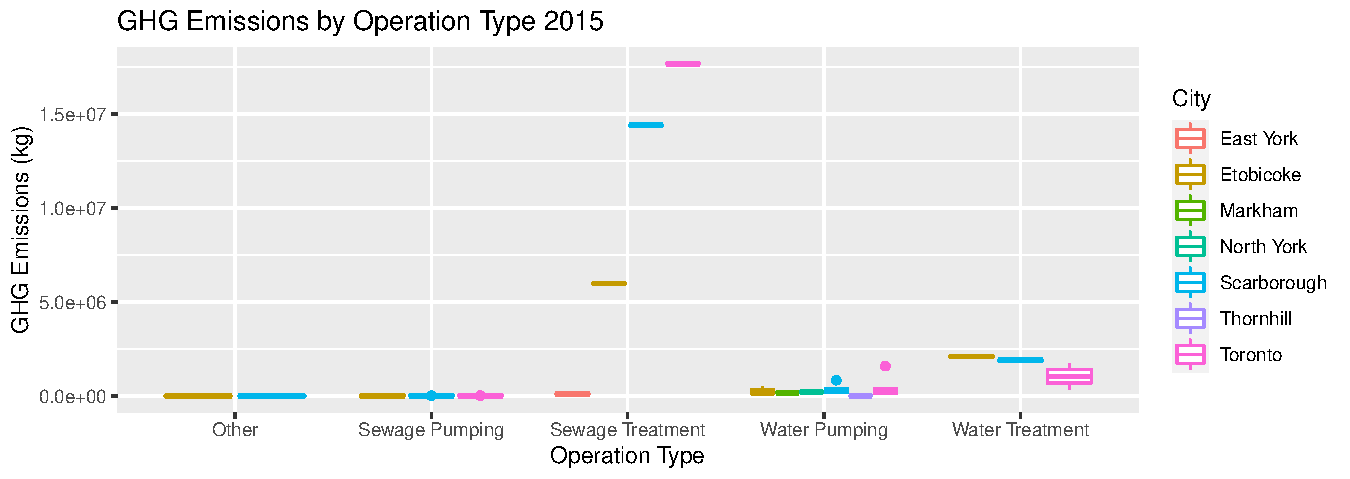
\includegraphics{paper_files/figure-pdf/unnamed-chunk-4-1.pdf}

}

\caption{Figure 1: GHG Emissions for 2015 by Operation Type}

\end{figure}

\begin{figure}

{\centering 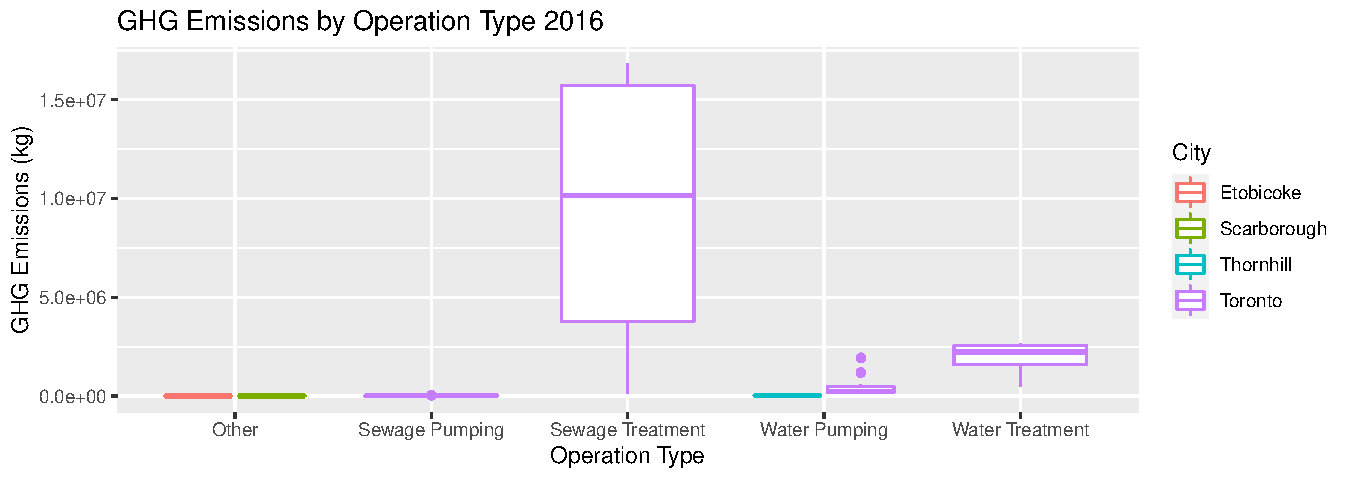
\includegraphics{paper_files/figure-pdf/unnamed-chunk-6-1.pdf}

}

\caption{Figure 2: GHG Emissions for 2016 by Operation Type}

\end{figure}

\begin{figure}

{\centering 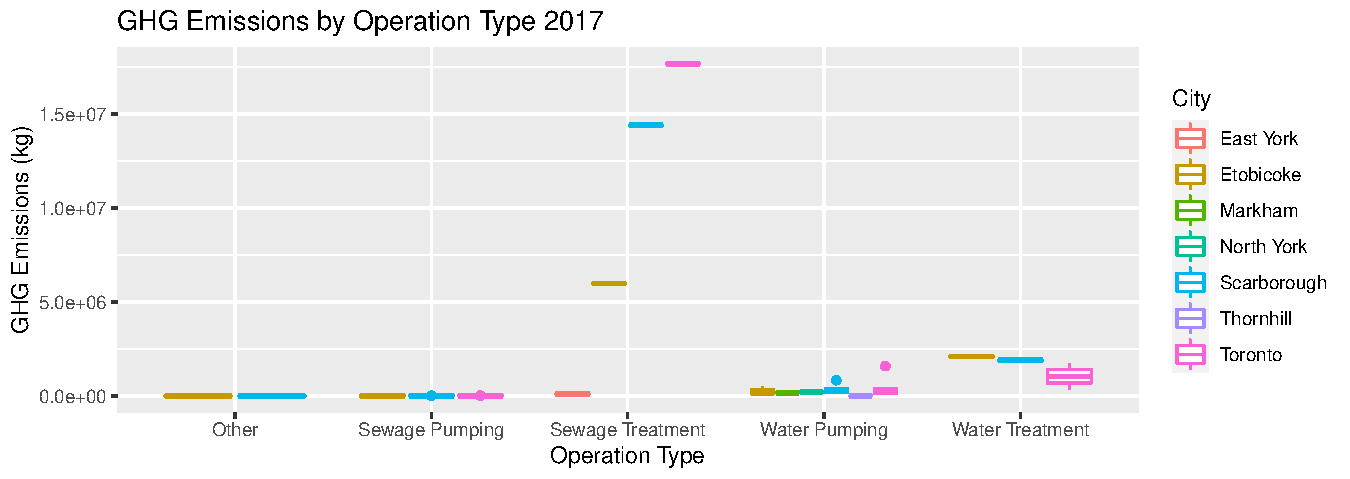
\includegraphics{paper_files/figure-pdf/unnamed-chunk-8-1.pdf}

}

\caption{Figure 3: GHG Emissions for 2017 by Operation Type}

\end{figure}

\begin{figure}

{\centering 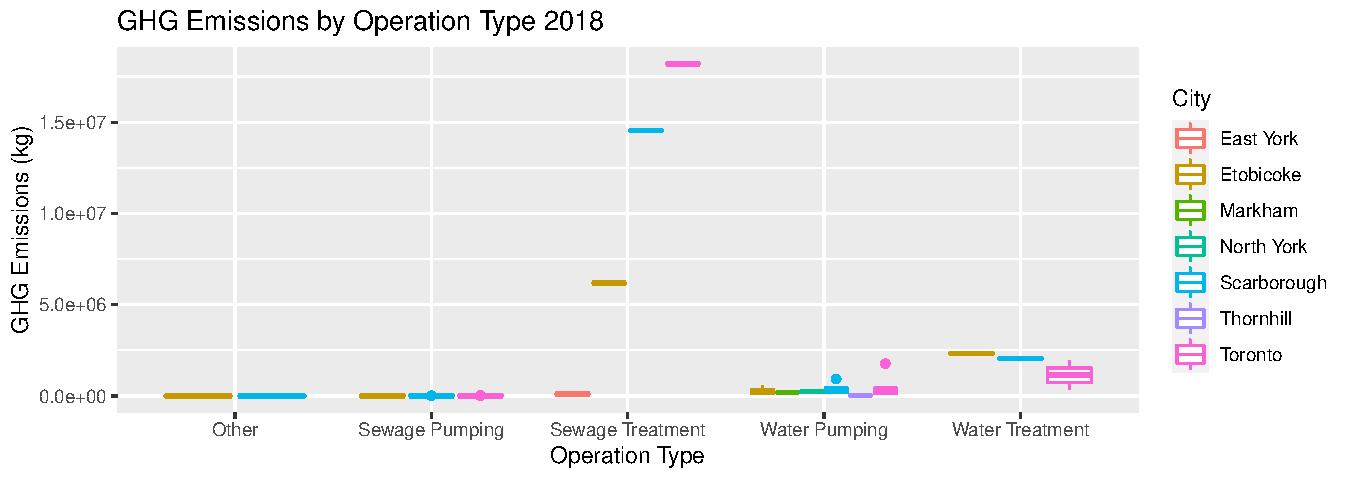
\includegraphics{paper_files/figure-pdf/unnamed-chunk-10-1.pdf}

}

\caption{Figure 4: GHG Emissions for 2015 by Operation Type}

\end{figure}

As seen in Figures 1 to 4, there are drastic changes in GHG emissions by
operation type and city from 2015 to 2018. From 2015 to 2016, GHG
emissions were the most in Toronto for the sewage treatment operation,
and the second highest was Toronto for the water treatment operation.
Both 2015 and 2016 had these results.

In 2017, the graph changes drastically. It can be observed that Toronto
still had some of the highest GHG emissions for the sewage treatment
operation but not nearly as much as it was before. The same can be seen
in 2018.

Next Steps

After analyzing this data set, it can be observed that the GHG emissions
are still very high throughout the GTA and there should be efforts to
reduce these emissions. There should be further analysis done on the
sewage and water treatment operations to find out what has been causing
the high GHG emissions for these operations.



\end{document}
